%%
%% Arquivo principal
%%

\documentclass[letterpaper,12pt,openright,twoside]{book}

\usepackage[latin1]{inputenc}
\usepackage[T1]{fontenc}
\usepackage{times}
\usepackage[portuges, brazil]{babel}    % hiphena��o em portugues
\usepackage{indentfirst}        % indenta primeiro par�grafo
\usepackage{graphicx}
\usepackage{fancyhdr}
\usepackage{wasysym}
\usepackage{pifont}
\usepackage{textcomp}      % \texttrademark
\usepackage{nomencl}    % glossario
\usepackage{url}  
\usepackage{multirow}  
%\usepackage[round]{natbib}  % cita��es tipo  (nome-ano)
%\usepackage{natbib}  % cita��es tipo  [nome-ano]
\usepackage[alf]{abntcite} % cita��es no formato abnt
\usepackage{setspace}

%% tamanho do texto e margens
\headheight 16pt
\setlength{\topmargin}{-15pt} % extra vert. space + at the top of header: 23pt
\setlength{\oddsidemargin}{0pt} % extra spc added at the left of odd page: 0pt
\setlength{\evensidemargin}{-12pt} % ext. spc added at the left of even pg: 59pt
\setlength{\textheight}{638pt} % height of the body: 592pt
\setlength{\textwidth}{483pt} % width of the body: 470pt

%% Estilo da p�gina corrente e demais p�ginas
\pagestyle{fancyplain}
\renewcommand{\chaptermark}[1]{\markboth{#1}{}}
\renewcommand{\sectionmark}[1]{\markright{\thesection\ #1}}
\lhead[\fancyplain{}{\bfseries\thepage}]{\fancyplain{}{\bfseries\rightmark}}
\rhead[\fancyplain{}{\bfseries\leftmark}]{\fancyplain{}{\bfseries\thepage}}
\cfoot[\fancyplain{\bfseries\thepage}{}]{\fancyplain{\bfseries\thepage}{}}

% Lista de arquivos a serem processados
\includeonly{capa,resumos2,Cap1/cap1,ApendiceA/apA}

%% Para a cria��o do Gloss�rio
\makenomenclature

%% Comandos para facilitar a edi��o 
\newcommand{\cpp}{\texttt{C$++$}}
\newcommand{\latex}{\LaTeX}


%% Inicia o texto
\begin{document}

%% Abrevia figuras e tabelas
\def\figurename{Fig.}
\def\tablename{Tab.}

%% Paginas iniciais (sem numera��o)
\frontmatter

%% P�gina de rosto
%%
%% ********** P�gina de Rosto
%%

%% n�o numerar a p�gina
\thispagestyle{empty}

\begin{center}
{\large Nome da Disciplina ou Autor}
 
\vspace{0.9in}
{\Large \textbf{Primeira Linha do T�tulo}} \\ \vspace{2ex}
{\Large \textbf{Segunda Linha do T�tulo}} \\

\vspace{2in}
\begin{flushright}
\parbox{3.50in}{
Informa��es adicionais}
\end{flushright}

\vspace{0.2in}
\begin{flushright}
\parbox{3.50in}{Autor 1 \\ 
Autor 2}
\end{flushright}


\vspace{1.2in}
Campinas, SP \\
2009
\end{center}





%% Resumo/Abstract
%%
%% ********** Resumo
%%
\newpage \thispagestyle{plain} 
\vspace{1.5cm}
\begin{center}
{\huge{\textbf{Resumo}}}
\end{center}
\vspace{0.5cm}

O resumo deve apresentar ao leitor uma id�ia compacta, mas clara
do trabalho descrito na tese. A defini��o precisa e import�ncia do problema
abordado, os principais objetivos, motiva��es e desafios da pesquisa s�o bons pontos 
de partida para o resumo. A estrat�gia ou metodologia empregada 
na pesquisa, suas principais contribui��es e os resultados
mais importantes tamb�m devem fazer parte do resumo. Note que tanto 
o resumo quanto o {\it abstract} devem compartilhar a mesma p�gina.

\vspace{1.5ex}

{\bf Palavras-chave}: Processamento de texto, \latex,
Prepara��o de Teses, Relat�rios T�cnicos.

%%
%% ********** Abstract
%%

\vspace{1.5cm}
\begin{center}
{\huge{\textbf{Abstract}}}
\end{center}
\vspace{0.5cm}

The abstract must present to the reader a short, but clear idea
of the work being reported in the thesis. The precise definition
and importance of the problem being addressed, the main objectives,
motivations and challenges of the research are a good starting point for the
abstract. The strategy or metodology employed
in the research, its main contributions, and the
most important results achieved may be part of the abstract as well. Notice 
that the {\it resumo} and the abstract must share the same
page.

\vspace{1.5ex}

{\bf Keywords}: Document Processing, \latex, Thesis Preparation,
Technical Reports.





%% Lista de conte�do (sum�rio)
\def\contentsname{Sum�rio}
\tableofcontents

%% Lista de figuras (gerada automaticamente)
\cleardoublepage
\addcontentsline{toc}{chapter}{Lista de Figuras}
\listoffigures

%% Lista de tabelas (gerada automaticamente)
\cleardoublepage
\addcontentsline{toc}{chapter}{Lista de Tabelas}
\listoftables

%% Gloss�rio (gerado automaticamente - veja entradas em cap1.tex)
\cleardoublepage
\renewcommand{\nomname}{Gloss�rio}
\markboth{GLOSS�RIO}{GLOSS�RIO}
\addcontentsline{toc}{chapter}{\nomname}
\printnomenclature

\mainmatter

%% Cap. 1 - Introdu��o
%%
%% Cap�tulo 1: Modelo de Cap�tulo
%%
\chapter{Modelo de cap�tulo}
\label{Cap:modelo}

O cap�tulo deve conter uma introdu��o e um fecho.
A introdu��o fornece ao leitor uma breve descri��o
do que ser� tratado no cap�tulo, enquanto o fecho
apresenta coment�rios finais sobre o que foi desenvolvido
no cap�tulo. 

Cap�tulos s�o divididos em se��es. O n�mero ideal de
se��es � imposs�vel de se precisar. Entretanto, um
cap�tulo com uma �nica se��o provavelmente deve ser
agregado ao cap�tulo anterior ou posterior. Um cap�tulo
com quinze se��es provavelmente deve ser subdividido em
dois cap�tulos.

Cap�tulos, se��es e subse��es devem ser rotulados para que 
possam ser  referenciados em qualquer parte do texto. 
Exemplo: $\ldots$ no cap�tulo~\ref{Cap:modelo} apresentamos
um modelo de cap�tulo de tese.


\section{Se��es}
\label{Sec:secoes}  %% labels n�o devem conter caracteres acentuados

Se��es s�o divis�es do conte�do do cap�tulo. Esta divis�o
deve ser l�gica (tem�tica) e n�o f�sica (por tamanho).
Por exemplo, um cap�tulo que trata de \textit{software}
de sistema teria se��es que tratam de montadores, ligadores,
carregadores, compiladores e sistemas operacionais.

Tal como cap�tulos, se��es devem ser rotuladas para refer�ncia
em outras partes do texto. Se��es s�o divididas em subse��es.

\subsection{Subse��es}
\label{Sec:subsecoes}

Subse��es s�o divis�es de se��es. No exemplo do texto sobre \textit{software}
de sistema, a se��o re\-fe\-ren\-te a sistema operacional conteria, 
por exemplo, subse��es que tratam de arquivos, processos, mem�ria e 
entrada/sa�da. Tal como se��es, subse��es s�o divis�es tem�ticas do texto.


\subsection*{Subsubse��es}
\label{Sec:subsubsecoes}

Subsubse��es s�o divis�es de subse��es e n�o devem ser numeradas no texto.
O $\ast$ ap�s o comando \textit{subsubsection} instrui o \latex~a n�o numerar
a subsubse��o.


\section{Figuras, tabelas e gr�ficos}
\label{Sec:figuras}

Figuras s�o editadas com editores gr�ficos capazes de exportar
a figura em formatos PS (\textit{PostScript}) 
ou, preferencialmente, EPS (\textit{Encapsulated PostScript}).
O editor \textit{xfig} � adequado para a maioria dos casos.
Por exemplo, a figura~\ref{fig:PNO-PrvSrv} foi editada no
\textit{xfig}. Outra op��o � o editor {\texttt dia}, um editor 
orientado a diagramas (UML, fluxograma, etc.) com capacidade de exportar 
EPS~\cite{hp-dia03}  Figuras em formato GIF, JPEG e bitmap podem ser
convetidas para o formato EPS atrav�s do aplicativo 
{\textit xv}. {\textit xv} n�o lista o formato EPS
dentre aqueles que � capaz de manipular. Entretanto,
selecionando-se o formato \textit{PostScript} e fornecendo-se
a extens�o {\textit .eps} ao nome do arquivo, o formato
EPS � gerado.


\begin{figure}[!hbt]
\centering 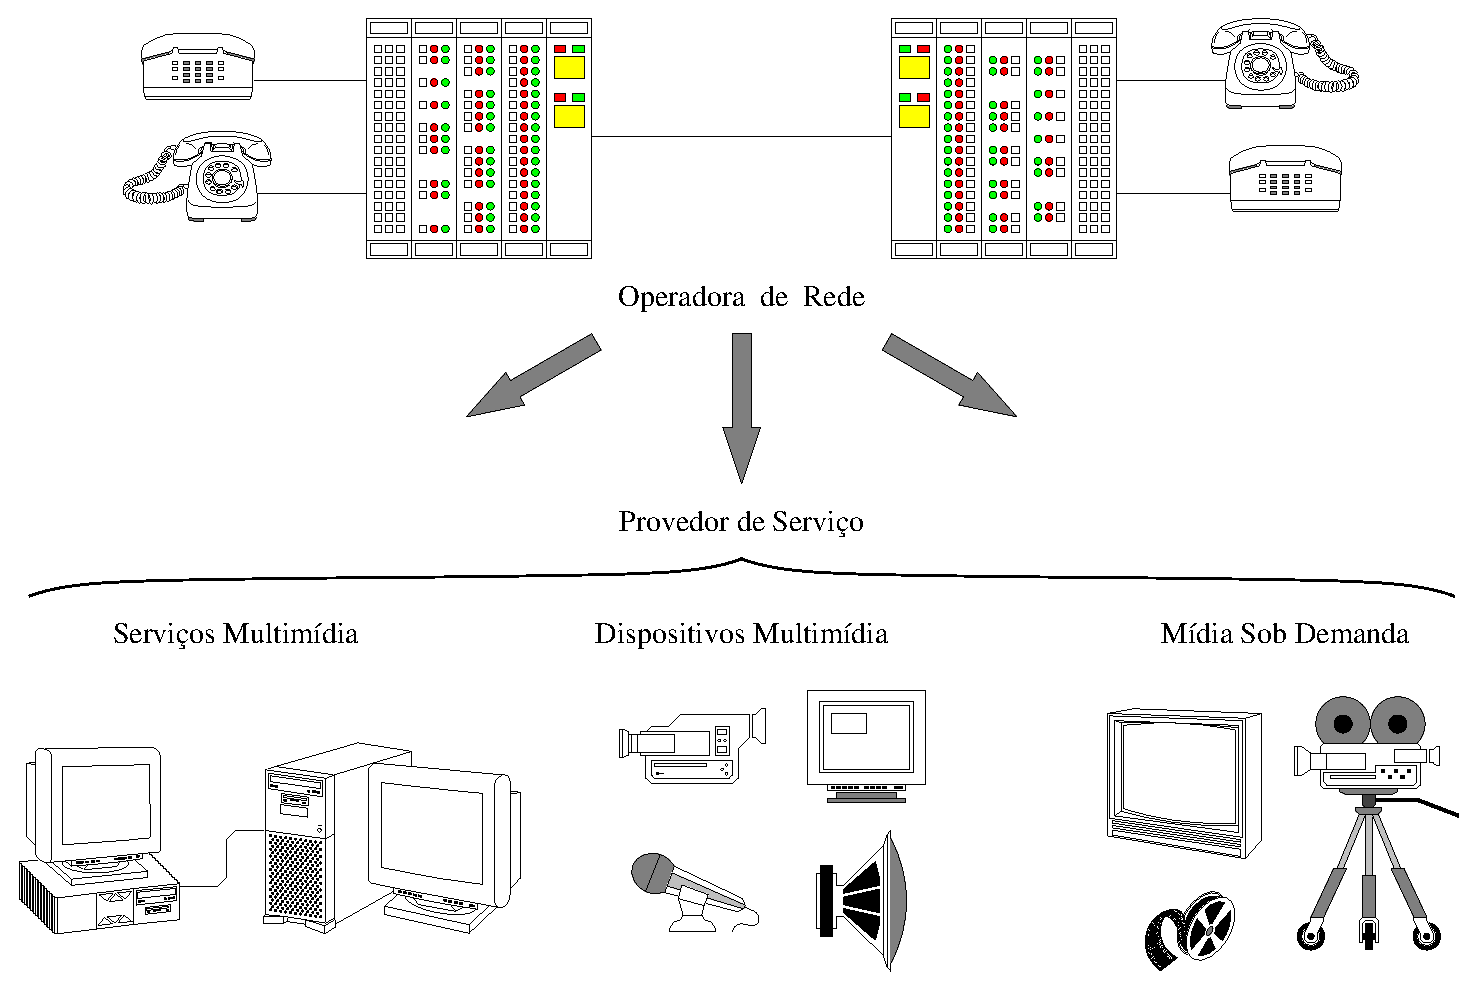
\includegraphics[width=12cm]{{./Cap1/pno-retl.eps}}
\caption{Operador de rede - provedor de servi�o.}
\label{fig:PNO-PrvSrv}
\end{figure}

Tabelas s�o constru�das com comandos pr�prios do \latex. Por
exemplo, a tabela~\ref{tab:Cmpt-SessAcss-ArchServ} foi constru�da desta forma.

\begin{table}[!htb]  \begin{center} 
\begin{tabular}{|c|c|l|c|} \hline\hline
\textit{Categoria} & \textit{Dom�nio} & \textit{Componente} & \textit{Acr�nimo}
 \\ \hline\hline
\multirow{5}{4cm}{Sess�o de Acesso} & \multirow{2}{2cm}{Usu�rio} &
 Aplica��o do Usu�rio & asUAP \\ \cline{3-4}
  & & Agente do Provedor   & PA \\ \cline{2-4}
  & \multirow{3}{2cm}{Provedor} & Agente do Usu�rio & UA \\ \cline{3-4}
  & & Agente de Usu�rio Especificado & namedUA \\ \cline{3-4}
  & & Agente de Usu�rio An�nimo & anonUA \\ \hline\hline
\end{tabular} 
\end{center}
\caption{Componentes da sess�o de acesso da arquitetura de servi�o TINA.}
\label{tab:Cmpt-SessAcss-ArchServ}
\end{table}


Gr�ficos s�o gerados com aplicativos capazes de exportar
nos formatos PS ou EPS. A ferramenta \textit{gnuplot} �
uma das mais utilizadas para a gera��o de gr�ficos. 
Uma vez no formato EPS, gr�ficos s�o inseridos no texto
tal como figuras (vide figura~\ref{fig:PbmDiversos}).


\begin{figure}[!hbt]
\centering 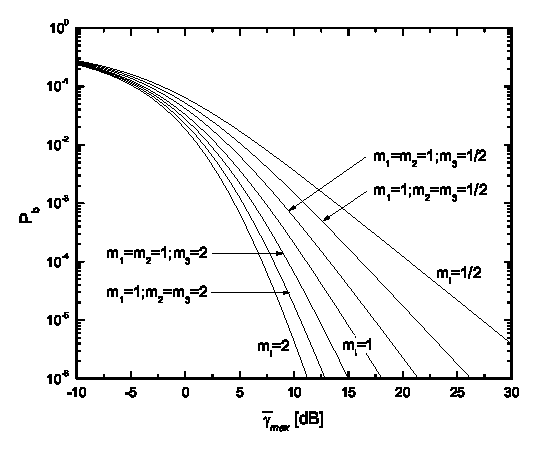
\includegraphics[width=.7\linewidth]{./Cap1/PbmDiversos.eps}
\caption{$P_b$; desvanecimentos arbitr�rios~\mbox{($M=3$).}}
\label{fig:PbmDiversos}
\end{figure}


\section{Cita��es bibliogr�ficas}
\label{Sec:citacoes}

\latex~utiliza um arquivo em separado para as refer�ncias bibliogr�ficas.
Este arquivo deve possuir o mesmo nome do arquivo mestre com a extens�o \textit{bib}.
Arquivos \textit{bib} possuem os seguintes estilos de refer�ncia:
\begin{itemize} \itemsep -0.5ex
\item artigos em anais de simp�sios~\cite{proc-faina01};
\item artigos em colet�neas de artigos~\cite{col-pinto00};
\item cap�tulos de livros~\cite{inbook-santos00};
\item anais de simp�sios~\cite{proc-sbrc02};
\item livros~\cite{book-lamport94};
\item teses de doutorado~\cite{phd-faina01};
\item teses de mestrado~\cite{msc-santos03};
\item relat�rios t�cnicos~\cite{rep-omg2000};
\item manuais t�cnicos~\cite{man-orbix99};
\item trabalhos n�o publicados~\cite{unp-sichman02};
\item p�ginas na Internet~\cite{hp-dia03} (utilizar como data a data do �ltimo acesso � p�gina);
\item miscel�nea~\cite{misc-cruz03}.
\end{itemize}


\section{Equa��es}
\label{Sec:equacoes}

\latex~� insuper�vel no processamento de equa��es. Equa��es
simples como $2^{n}$ podem ser editadas no pr�prio texto.
Equa��es complexas como


\begin{eqnarray} \label{eq:PDF:RSR}
  p \left( \gamma \right) & = & \frac{1}{2} \sqrt{\frac{M}{\gamma \bar{\gamma}_{b}}} \frac{1}{ \prod_{i=1}^M {\sqrt{\tilde{\gamma}_i}}}
  \int_0^{\sqrt{M \delta}} \int_0^{\sqrt{M \delta} - r_M } \cdots
  \int_0^{\sqrt{M \delta} - \sum_{i = 3}^M {r_i } } \nonumber \\
  & & p \left( {\frac{\sqrt{M \delta} - \sum_{i = 2}^M {r_i }}{\sqrt{\tilde{\gamma}_1}} ,
  \frac{r_2}{\sqrt{\tilde{\gamma}_2}} , \ldots ,\frac{r_M}{\sqrt{\tilde{\gamma}_M}} } \right)
  \, dr_2 \cdots dr_{M-1} \, dr_M
\end{eqnarray}

ou


\begin{equation}\label{eq:TrCGI}
  T(r) = \frac{1}{f_m}
  \left( \frac{\pi}{2} \sum_{i=1}^M
  {\tilde{r}_i^2 \dot{\varsigma}_i^2}\right)^{-1/2}
  \frac
  {\begin{array}{ll}
  \int_0^{\rho \sqrt{M}} \int_0^{\rho \sqrt{M} - r_M } \cdots
  \int_0^{\rho \sqrt{M} - \sum_{i = 3}^M {r_i } } \int_0^{\rho \sqrt{M} -
  \sum_{i = 2}^M {r_i } }  \\
  p \left( {\frac{r_1}{\tilde{r}_1} ,
  \frac{r_2}{\tilde{r}_2} , \ldots ,\frac{r_M}{\tilde{r}_M} } \right)
  \, dr_1 \, dr_2 \cdots dr_{M-1} \, dr_M \\ \end{array}}
  {\begin{array}{ll}
  \int_0^{\rho \sqrt{M}} \int_0^{\rho \sqrt{M} - r_M } \cdots
  \int_0^{\rho \sqrt{M} - \sum_{i = 3}^M {r_i } } \\
  p \left( {\frac{\rho \sqrt{M} - \sum_{i = 2}^M {r_i }}{\tilde{r}_1} ,
  \frac{r_2}{\tilde{r}_2} , \ldots ,\frac{r_M}{\tilde{r}_M} } \right)
  \, dr_2 \cdots dr_{M-1} \, dr_M \\ \end{array}}
\end{equation}

\noindent
s�o automaticamente numeradas e podem ser referenciadas a partir do
texto. Por exemplo, a equa��o~\ref{eq:TrCGI} � trivialmente derivada
da equa��o~\ref{eq:PDF:RSR}.



\section{Gloss�rio}
\label{Sec:glossario}

\latex~gera automaticamente o gloss�rio. Ao redigir uma sigla pela primeira vez, o
autor, ao final do par�grafo, gera a entrada para o gloss�rio. Exemplo:

A camada de adapta��o tipo 1 (ATM AAL1) das redes digitais de servi�os integrados em
faixa larga (B-ISDN) � especificada pela ITU-T.
\nomenclature{ATM - }{Asynchronous Transfer Mode}
\nomenclature{AAL1 - }{ATM Adaptation Layer Type 1}
\nomenclature{B-ISDN - }{Broadband Integrated Service Digital Network}
\nomenclature{ITU-T - }{International Telecommunication Union-Telecommunication Standardization Sector}


\section{Estilo}
\label{Sec:estilo}

Recomenda-se espa�amento 1.5 entre as linhas do texto.
Evite sempre os seguintes recursos (ou melhor, enfeites):
\begin{itemize}
\item \textbf{o uso de negrito;}
\item \textit{o uso de it�lico (exceto em palavras em outra l�ngua);}
\item \texttt{texto em diferente fonte como m�quina de escrever;}
\item \underline{o uso de texto sublinhado;}
\item o uso excessivo de~\footnote{Notas de rodap�.}.
\end{itemize}

Lembre-se: um texto ``limpo'' � mais agrad�vel de ler que um texto ``enfeitado''.




%% Refer�ncias bibliog�ficas (geradas automaticamente)
\addcontentsline{toc}{chapter}{Refer�ncias bibliogr�ficas}
%\bibliographystyle{plainnat}  %% nome-ano
%\bibliographystyle{unsrt}    %% numero
\bibliographystyle{abnt-alf}  %% nome-ano
\bibliography{monografia}

\appendix
%%Ap�ndice A 
\chapter{Ap�ndices}

No \latex~ap�ndices s�o editados como cap�tulos. O comando \textit{apendix} 
(vide arquivo mestre) faz com que todos os cap�tulos seguintes sejam
considerados ap�ndices.

Ap�ndices complementam o texto principal da tese com informa��es
para leitores com especial interesse no tema, devendo ser considerados
leitura opcional, ou seja, o entendimento do texto principal da tese
n�o deve exigir a leitura atenta dos ap�ndices.

Ap�ndices usualmente contemplam provas de teoremas, dedu��es 
de f�rmulas matem�ticas, diagramas esquem�ticos, gr�ficos e
trechos de c�digo. Quanto a este �ltimo, c�digo extenso n�o
deve fazer parte da tese, mesmo como ap�ndice. O ideal
� disponibilizar o c�digo na Internet para os interessados
em examin�-lo ou utiliz�-lo.


\end{document}

